\documentclass[tikz,border=3mm]{standalone}
\begin{document}
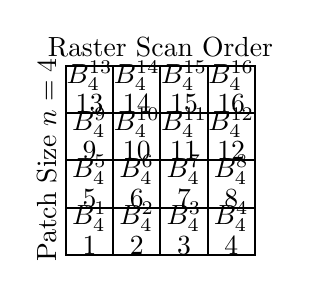
\begin{tikzpicture}[scale=1.2]
  % Grid lines (optional, for structure reference)
  \draw[gray!30,thin] (0,0) grid[step=0.5] (2,2);
  \draw[gray!30,thin] (0,0) grid[step=0.5] (2,2); % Double grid for clarity
  
  % Blocks and labels
  \foreach \row in {0,...,3} {
    \foreach \col [evaluate=\col as \i using int(\row*4+\col+1)] in {0,...,3} {
      % Block rectangle
      \draw[thick] (\col*0.5, \row*0.5) rectangle (\col*0.5+0.5, \row*0.5+0.5);
      
      % Block label (top) and sequence number (bottom)
      \node at (\col*0.5+0.25, \row*0.5+0.4) {\( B_4^{\i} \)};
      \node at (\col*0.5+0.25, \row*0.5+0.1) {\i};
    }
  }
  
  % Axes labels (optional)
  \node[above] at (1,2) {Raster Scan Order};
  \node[left] at (0,1) {\rotatebox{90}{Patch Size \( n=4 \)}};
\end{tikzpicture}
\end{document}